 \documentclass[12pt,a4paper]{report} %set default font to 12 and change to report

\usepackage{amsmath}
\usepackage{amssymb}
\usepackage{amsthm}
\usepackage{color}
\usepackage{algorithm}
\usepackage{algorithmic}
\usepackage{graphicx}
\usepackage{multirow}
\usepackage[title,titletoc]{appendix}
\usepackage{vector}
\usepackage{titletoc}
\usepackage{enumitem}
\usepackage{setspace} % for switching between double/single space in document
\usepackage{fancyhdr} % package for changing Headings style
\usepackage{fontspec}
\usepackage[labelsep=space,width=\hsize,format=hang,font=footnotesize,labelfont=bf]{caption}
\usepackage[labelsep=space, subrefformat=parens, width=\hsize]{subfig}
\usepackage[Kashida]{xepersian}

% این دستور به منظور تنظیم اندازهصفحه قرار داده شده است
%\usepackage[paperwidth=210mm,paperheight=297mm]{geometry} %setting the page size

% setting the margins of page
\usepackage[top=2.5cm,right=2cm,bottom=2.5cm,left=2cm]{geometry}


% tell tex engine address of folder containing your pictures
\graphicspath{{images/}}

\bibliographystyle{unsrt}

\algsetup{
   linenosize=\small,
   linenodelimiter=)
}


\relpenalty=10000
\binoppenalty=10000


% تغییر و ساخت فونت های مناسب
\defpersianfont\BKoodakpart[Scale=1.3]{B Koodak} 
\defpersianfont\BKoodakchapter[Scale=1.2]{B Koodak} 
\defpersianfont\BKoodaksection[Scale=1.1]{B Koodak} 
\defpersianfont\BKoodak[Scale=1.0]{B Koodak} 


\settextfont[Scale=1.18]{B Koodak}
\setsansfont[Scale=1.0]{Times New Roman}
% تغییر به فونت  11
\setlatintextfont[Scale=1.0]{Times New Roman}
\setdigitfont[Scale=1.2]{PGaramond}

% تنظیم فاصله ی بین خطوط
\renewcommand{\baselinestretch}{0.7}%setting the space between lines


\DeclareMathSizes{10}{12}{10}{8}
% -------------------------------------

%\def\listfigurename{فهرست اشکال}
%\def\listtablename{فهرست جداول}
%\def\bibname{\rl{مراجع}}


\titlecontents{chapter}[1cm]
  {\bfseries\addvspace{5pt}}
  {\hspace*{-1cm}\bfseries\textsc{\chaptertitlename}\thecontentslabel-\hspace{5pt}}
  {\hspace*{-1cm}}
  {\hfill\contentspage}



\setenumerate[1]{label=\arabic*), ref=\arabic*}

\setcounter{secnumdepth}{4}
\setcounter{tocdepth}{2}

%تغییر فونت  part ها به لوتوس ساه زده شده است 
\title{\BKoodakpart {گزارش جلسه سوم آزمایشگاه پایگاه داده}}%change font to b Koodak 20 as defined before
\author{سامان فکری 9231075
			\and سجاد اعظمی 9231031}

%\renewcommand{\contentsname}{سوالات}

\begin{document}

\Persian
\maketitle

%\tableofcontents
%\contentsline {chapter}{\title {سوال 1}}{3}
\contentsline {section}{\title{الف)}}{3}
\contentsfinish 
%\listoffigures
\newpage
%\listoftables

\Persian 

\chapter*{\title\BKoodakchapter{سوال 1}}%change font to b Koodak 13 as defined before
با استفاده از دستورات زیر جدول خواسته شده را می سازیم.
\begin{figure}[h!]
\centering
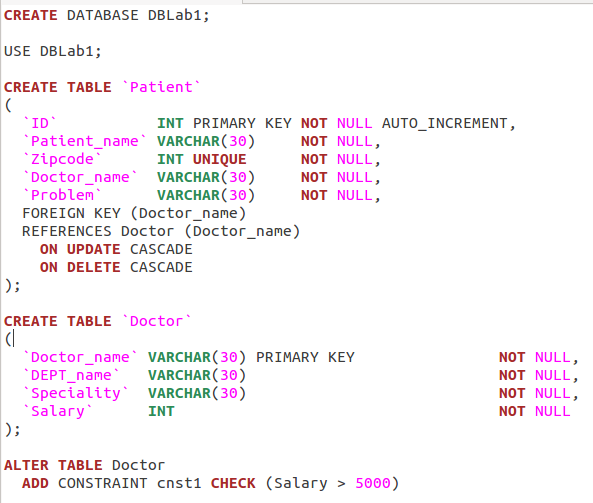
\includegraphics[width=.9\textwidth]{pics/1.png}
\end{figure}

\section*{\BKoodaksection{الف)}}
در این قسمت با استفاده از دستورات زیر افراد را برحسب نام خانوادگی به ترتيب صعودی مرتب می کنیم.
\begin{figure}[h!]
\centering
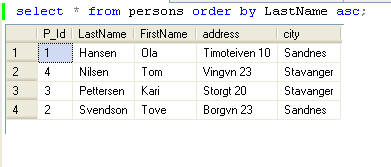
\includegraphics[width=.9\textwidth]{pics/3.png}
\end{figure}
\newpage

\section*{\BKoodaksection{ب)}}
با استفاده از دستور زیر یک فیلد به جدول اضافه می کنیم و یک شرط روی آن فیلد می گذاریم.
\begin{figure}[h!]
\centering
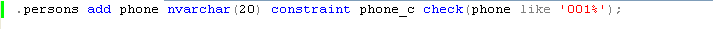
\includegraphics[width=.9\textwidth]{pics/4-1.png}
\end{figure}
سپس با تراکنش زیر اطلاعات شماره تلفن را به جدول اضافه می کنیم
\begin{figure}[h!]
\centering
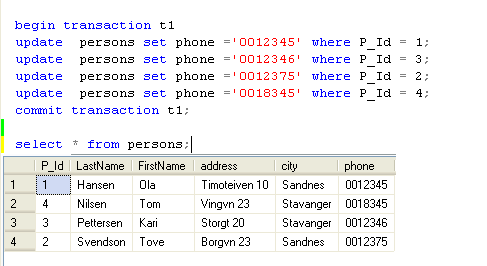
\includegraphics[width=.9\textwidth]{pics/4.png}
\end{figure}

\section*{\BKoodaksection{پ)}}
با استفاده از دستور آدرس ها را به دلخواه نشان می دهیم.
\begin{figure}[h!]
\centering
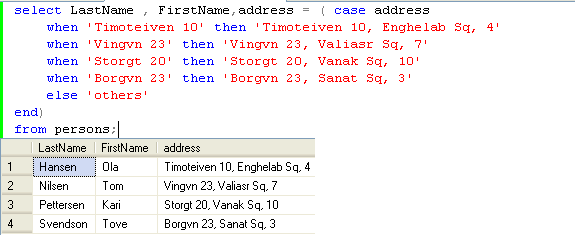
\includegraphics[width=.9\textwidth]{pics/5.png}
\end{figure}
\newpage

\section*{\BKoodaksection{ت)}}
با استفاده از دستور زیر شخصی را به جدول با یک تراکنش اضافه کردیم و مشخصه ی آن به اجبار 7 وارد شده است.
\begin{figure}[h!]
\centering
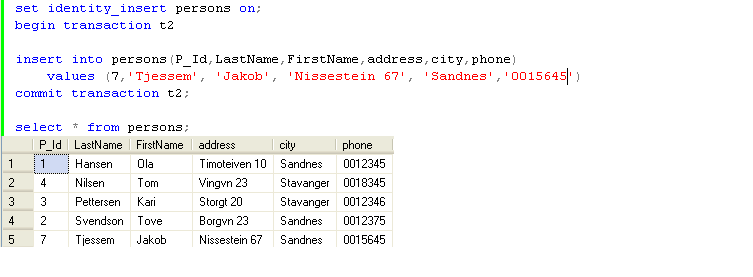
\includegraphics[width=.9\textwidth]{pics/6.png}
\end{figure}

\section*{\BKoodaksection{ث)}}
همه ی اشخاص خواسته شده بعد از 10 ثانیه نشان داده شده اند
\begin{figure}[h!]
\centering
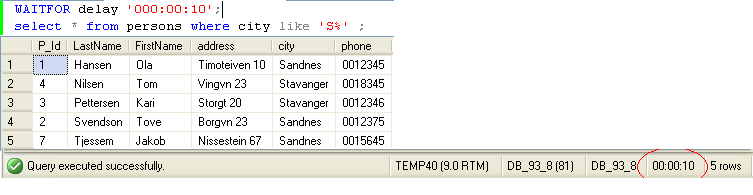
\includegraphics[width=.9\textwidth]{pics/7.png}
\end{figure}
\newpage
\section*{\BKoodaksection{ج)}}
روال آن به صورت زیر است.
\begin{figure}[h!]
\centering
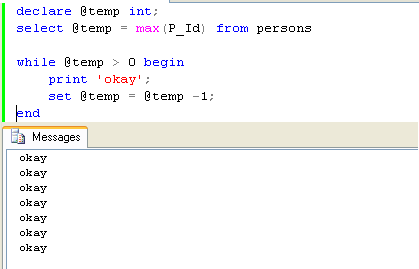
\includegraphics[width=.9\textwidth]{pics/8.png}
\end{figure}

\section*{\BKoodaksection{چ)}}
شماره تلفن که داده شده بزرگتر بوده است.
\begin{figure}[h!]
\centering
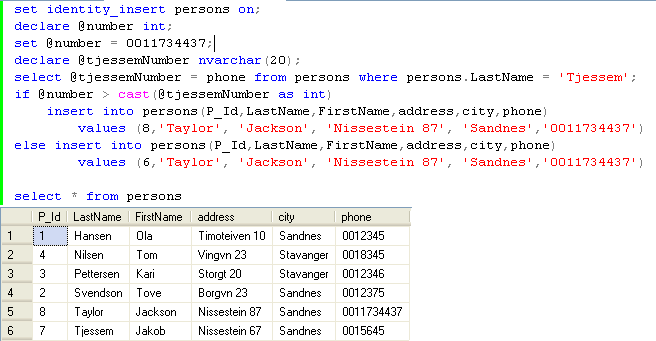
\includegraphics[width=.9\textwidth]{pics/9.png}
\end{figure}
\newpage

\chapter*{\title\BKoodakchapter{سوال 2}}%change font to b Koodak 13 as defined before
ابتدا جدول را ساخته و مقادیر را به آن اضافه می کنیم
\begin{figure}[h!]
\centering
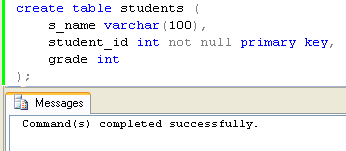
\includegraphics[width=.8\textwidth]{pics/10.png}
\end{figure}

\begin{figure}[h!]
\centering
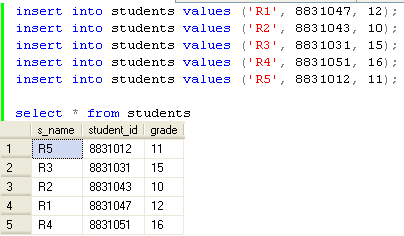
\includegraphics[width=.8\textwidth]{pics/11.png}
\end{figure}
\newpage
با استفاده از این دستور نمرات کسانی که زیر 15 بود را دو نمره اضافه کردیم .
\begin{figure}[h!]
\centering
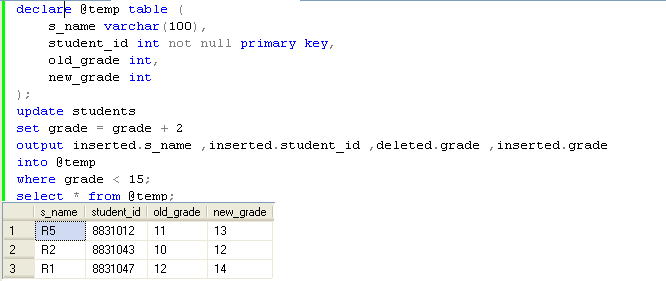
\includegraphics[width=1.0\textwidth]{pics/12.png}
\end{figure}
\newpage

\end{document}

